\begin{figure}[htbp]
\centering
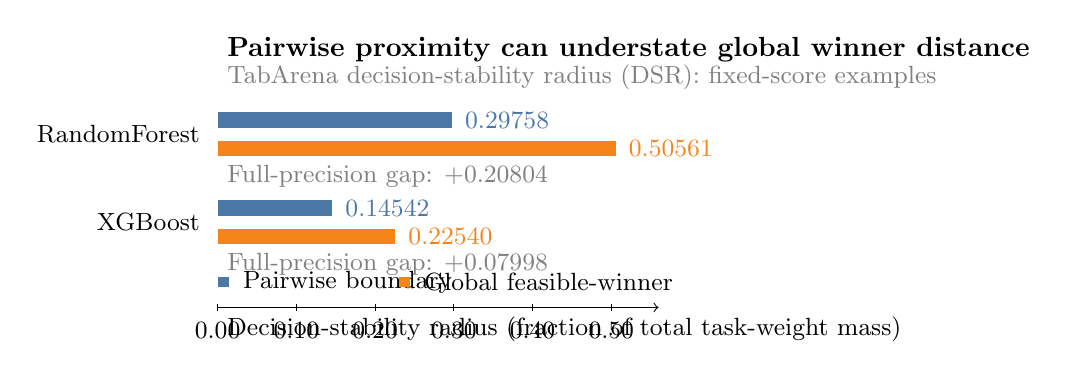
\begin{tikzpicture}[x=10cm,y=0.8cm,font=\small]
  \definecolor{pairblue}{RGB}{76,120,168}
  \definecolor{globalorange}{RGB}{245,133,24}

  \node[anchor=west,font=\bfseries] at (0,4.5) {Pairwise proximity can understate global winner distance};
  \node[anchor=west,text=gray] at (0,4.05) {TabArena decision-stability radius (DSR): fixed-score examples};

  \draw[->] (0,0.4) -- (0.56,0.4);
  \foreach \x/\lab in {0/0.00,0.1/0.10,0.2/0.20,0.3/0.30,0.4/0.40,0.5/0.50}
    {\draw (\x,0.35)--(\x,0.45) node[below=3pt] {\lab};}

  \node[anchor=east] at (-0.01,3.15) {RandomForest};
  \fill[pairblue] (0,3.25) rectangle (0.29758,3.50);
  \fill[globalorange] (0,2.80) rectangle (0.50561,3.05);
  \node[anchor=west,text=pairblue] at (0.302,3.375) {0.29758};
  \node[anchor=west,text=globalorange] at (0.510,2.925) {0.50561};
  \node[anchor=west,text=gray] at (0,2.48) {Full-precision gap: +0.20804};

  \node[anchor=east] at (-0.01,1.75) {XGBoost};
  \fill[pairblue] (0,1.85) rectangle (0.14542,2.10);
  \fill[globalorange] (0,1.40) rectangle (0.22540,1.65);
  \node[anchor=west,text=pairblue] at (0.150,1.975) {0.14542};
  \node[anchor=west,text=globalorange] at (0.230,1.525) {0.22540};
  \node[anchor=west,text=gray] at (0,1.08) {Full-precision gap: +0.07998};

  \fill[pairblue] (0,0.72) rectangle (0.015,0.88);
  \node[anchor=west] at (0.02,0.80) {Pairwise boundary};
  \fill[globalorange] (0.23,0.72) rectangle (0.245,0.88);
  \node[anchor=west] at (0.25,0.80) {Global feasible-winner};

  \node[anchor=west] at (0,0.05) {Decision-stability radius (fraction of total task-weight mass)};
\end{tikzpicture}
\caption{Pairwise versus global feasible-winner decision-stability radii for two TabArena challengers. Global feasibility can require additional task-weight redistribution beyond pairwise contact with the nominal winner. Endpoint labels are rounded; gap annotations use the stored full-precision radii.}
\label{fig:pairwise-global}
\end{figure}

